\PassOptionsToPackage{xetex}{xcolor}
\PassOptionsToPackage{xetex}{graphicx}
\documentclass[a4paper,landscape,headrule,footrule,xetex]{foils}


%%
%%% macros for 2009 Semester 1 HG 803
%%%
\newcommand{\logo}{~}
\newcommand{\header}[3]{%
  \title{\vspace*{-2ex} \large HG3051  Corpus Linquistics
    \\[2ex] \Large  \emp{#2} \\ \emp{#3}}
  \author{\blu{Francis Bond}   \\ 
    \normalsize  \textbf{Division of Linguistics and Multilingual Studies}\\
    \normalsize  \url{http://www3.ntu.edu.sg/home/fcbond/}\\
    \normalsize  \texttt{bond@ieee.org}}
  \MyLogo{HG3051 (2020)}
  \renewcommand{\logo}{#2}
  \hypersetup{
    pdfinfo={
      Author={Francis Bond},
      Title={#1: #2},
      Subject={HG3051: Corpus Linguistics},
      Keywords={Corpus Linguistics},
      License={CC BY 4.0}
    }
  }
  \date{#1 \\ \url{https://github.com/bond-lab/Corpus-Linguistics}}
}

\usepackage{fontenc}
\usepackage{polyglossia}
\setmainlanguage{english}
\setmainfont{TeX Gyre Pagella}
%\setmainfont{Linux Libertine}
%\setmainfont{Charis SIL}
\newfontfamily{\ipafont}{Gentium}
\newcommand{\ipa}[1]{{\ipafont\selectfont #1}}
\usepackage{xeCJK}

\setCJKmainfont{Noto Sans CJK SC}
\setCJKsansfont{Noto Sans CJK SC}
\newcommand{\zh}[1]{#1}
\makexeCJKinactive

\usepackage{xcolor}
\usepackage{graphicx}
\newcommand{\blu}[1]{\textcolor{blue}{#1}}
\newcommand{\grn}[1]{\textcolor{green}{#1}}
\newcommand{\hide}[1]{\textcolor{white}{#1}}
\newcommand{\emp}[1]{\textcolor{red}{#1}}
\newcommand{\txx}[1]{\textbf{\textcolor{blue}{#1}}}
\newcommand{\lex}[1]{\textbf{\mtcitestyle{#1}}}

\usepackage{pifont}
\renewcommand{\labelitemi}{\textcolor{violet}{\ding{227}}}
\renewcommand{\labelitemii}{\textcolor{purple}{\ding{226}}}

\newcommand{\subhead}[1]{\noindent\textbf{#1}\\[5mm]}

\newcommand{\Bad}{\emp{\raisebox{0.15ex}{\ensuremath{\mathbf{\otimes}}}}}
\newcommand{\bad}{*}

\newcommand{\com}[1]{\hfill \textnormal{(\emp{#1})}}%
\newcommand{\cxm}[1]{\hfill \textnormal{(\txx{#1})}}%
\newcommand{\cmm}[1]{\hfill \textnormal{(#1)}}%

\usepackage{relsize,xspace}
\newcommand{\into}{\ensuremath{\rightarrow}\xspace}
\newcommand{\ent}{\ensuremath{\Rightarrow}\xspace}
\newcommand{\nent}{\ensuremath{\not\Rightarrow}\xspace}
\newcommand{\tot}{\ensuremath{\leftrightarrow}\xspace}
\usepackage{url}
\newcommand{\lurl}[1]{\MyLogo{\url{#1}}}

\usepackage{mygb4e}
\let\eachwordone=\itshape
\newcommand{\lx}[1]{\textbf{\textit{#1}}}

%\usepackage{times}
%\usepackage{nttfoilhead}
\newcommand{\myslide}[1]{\foilhead[-25mm]{\raisebox{12mm}[0mm]{\emp{#1}}}\MyLogo{\logo}}
\newcommand{\myslider}[1]{\rotatefoilhead[-25mm]{\raisebox{12mm}[0mm]{\emp{#1}}}}
%\newcommand{\myslider}[1]{\rotatefoilhead{\raisebox{-8mm}{\emp{#1}}}}

\newcommand{\section}[1]{\myslide{}{\begin{center}\Huge \emp{#1}\end{center}}}



\usepackage[lyons,j,e,k]{mtg2e}
\renewcommand{\mtcitestyle}[1]{\textcolor{teal}{\textsl{#1}}}
%\renewcommand{\mtcitestyle}[1]{\textsl{#1}}
\newcommand{\chn}{\mtciteform}
\newcommand{\cmn}{\mtciteform}
\newcommand{\iz}[1]{\textup{\texttt{\textcolor{blue}{\textbf{#1}}}}}
\newcommand{\rel}[1]{\textsc{\color{blue}{#1}}}
\newcommand{\wn}[3]{\lex{#1}\ensuremath{_{#2:#3}}}
\newcommand{\con}[1]{\textsc{#1}}
\newcommand{\gm}{\textsc}
\usepackage[normalem]{ulem}
\newcommand{\ul}{\uline}
\newcommand{\ull}{\uuline}
\newcommand{\wl}{\uwave}
\newcommand{\vs}{\ensuremath{\Leftrightarrow}~}
\usepackage[hidelinks]{hyperref}
\hypersetup{
     colorlinks,
     linkcolor={blue!50!black},
     citecolor={red!50!black},
     urlcolor={blue!80!black}
}
%%%
%%% Bibliography
%%%
\usepackage{natbib}
%\usepackage{url}
\usepackage{bibentry}
%%% From Tim
\newcommand{\WMngram}[1][]{$n$-gram#1\xspace}
\newcommand{\infers}{$\rightarrow$\xspace}

\usepackage{bibentry}
\renewcommand{\cite}{\bibentry}

\header{Lecture 6}{DIY Corpora,  Processing Raw Text, SQL}{}

\usepackage{pst-node}
\newcommand{\sa}[2]{\rnode{c#1}{\iz{#2}}}%\nodebox{c#1}}

%\usepackage{hieroglf}
\usepackage{wasysym}
%\newcommand{\grn}[1]{\textcolor{PineGreen}{#1}}
\newcommand{\ont}[1]{\textcolor{blue}{#1}}
\newcommand{\jcy}[1]{\textcolor{orange}{#1}}
\newcommand{\lxd}[1]{\textcolor{brown}{#1}}

\newcommand{\hinoki}{\grn{Hinoki}\xspace}
\newcommand{\lexeed}{\lxd{Lexeed}\xspace}
\newcommand{\jacy}{\jcy{JACY}\xspace}
\newcommand{\onto}{\ont{Ontology}\xspace}
%\newcommand{\itsdb}{\textsf{[incr tsdb()]}\xspace}
\newcommand{\GT}{Goi-Taikei\xspace}


\begin{document}
\bibliographystyle{apalike}
\nobibliography{abb,mtg,nlp,ling}
\maketitle


\myslide{Overview}

\begin{itemize} 
\item Revision  of Statistics
  \begin{itemize} 
  \item Frequency
  \item Corpus Statistics
  \item Collocations
\end{itemize}
\item DIY Corpora
\item Processing Raw Text
\item Structured Query Language
\end{itemize}
%%% 
%%% this changes each year, so keep separate
%%%
\include{schedule}

%%%
\section{Revision  of Statistics}
%%%


\myslide{Lexical statistics}
%Zipf 1949/1961, Baayen 2001, Evert 2004

\begin{itemize}
\item Statistical study of the frequency distribution of types
(words or other linguistic units) in texts
\item Try to gauge who confident we are in our results
\item Try to measure if things are more common than chance
\end{itemize}

\myslide{Zipf’s law}

\begin{itemize}
\item  Zipf’s (1949, 1965) famous law:

  \begin{equation}
    \label{eq:1}
    f(w) = \frac{C}{r(w)^a}\ \ \  \textnormal{or} \ \ \  f(w) \propto \frac{1}{r(w)}
  \end{equation}
\begin{itemize}
  \item With a = 1 and C =60,000, Zipf’s law predicts that:
\begin{itemize}
  \item most frequent word occurs 60,000 times
  \item second most frequent word occurs 30,000 times
  \item third most frequent word occurs 20,000 times
  \item and there is a long tail of 80,000 words with frequencies
  \item between 1.5 and 0.5 occurrences(!)
  \end{itemize}
\end{itemize}
\end{itemize}

\myslide{Applications of word frequency distributions}
\begin{itemize}
  \item Most important application: extrapolation of vocabulary
size and frequency spectrum to larger sample sizes
\begin{itemize}
  \item productivity (in morphology, syntax, \ldots)
  \item lexical richness
\\ (in stylometry, language acquisition, clinical linguistics, \ldots)
\item practical NLP (est. proportion of OOV words, typos, \ldots)
\end{itemize}
\item Direct applications of Zipf’s law in NLP
\begin{itemize}
  \item Population model for Good-Turing smoothing
  \item Realistic prior for Bayesian language modelling
  \end{itemize}
\end{itemize}


\myslide{Statistics \& language}
\begin{itemize}
\item Apply statistical procedure to linguistic problem
  \begin{itemize}
  \item take random sample from (extensional) language
  \item What are the objects in our population?
    \begin{itemize}
    \item words? sentences? texts? …
    \end{itemize}
  \item Objects = whatever proportions are based on
    \into unit of measurement
  \end{itemize}
\item We want to take a random sample of these units
\end{itemize}

 

\myslide{Inference from a sample}
\begin{itemize}
\item Principle of inferential statistics
\begin{itemize}
\item if a sample is picked at random, proportions should be
roughly the same in the sample and in the population
\end{itemize}
\item Take a sample of, say, 100 VPs
\begin{itemize}
\item observe 19 passives \into $p = 19\% = .19$
\item style guide \into population proportion $\pi = 15\%$
\item $p > \pi$ \into reject claim of style guide?
\end{itemize}
\item Take another sample, just to be sure
\begin{itemize}
\item observe 13 passives \into $p = 13\% = .13$
\item $p < \pi$ \into claim of style guide confirmed?
\end{itemize}
\end{itemize}

\myslide{Sampling variation}
\begin{itemize}
\item random choice of sample ensures proportions are the
  same on average in sample and in population
\item but it also means that for every sample we will get a
different value because of chance effects
\into sampling variation
\item The main purpose of statistical methods is to
estimate \& correct for sampling variation
\end{itemize}
\myslide{Estimating sampling variation}
\begin{itemize}
\item We don't need an infinite number of monkeys
(or corpus linguists) to answer these questions
\begin{itemize}
\item Statistical hypothesis tests
\begin{itemize}
\item define a rejection criterion for refuting $H_0$
\item control the risk of false rejection (type I error) to a
“socially acceptable level” (significance level)
\item p-value = risk of false rejection for observation
\item p-value interpreted as amount of evidence against $H_0$
\end{itemize}
\item Two-sided vs. one-sided tests
\begin{itemize}
\item in general, two-sided tests should be preferred
\item one-sided test is plausible in our example
\end{itemize}
\end{itemize}
\end{itemize}


\myslide{Hypothesis tests in practice}
\begin{itemize}
\item Easy: use online wizard
  \begin{itemize}
  \item \url{http://sigil.collocations.de/wizard.html}
  \item \url{http://faculty.vassar.edu/lowry/VassarStats.html}
  \item open-source software \url{http://www.r-project.org/}
\end{itemize}
\item Or Python
  \begin{itemize}
  \item One-tail test 
    \\ \texttt{scipy.stats.binom.sf(51-1, 235, 1.0/6)}
  \item Two-tail test
    \\ \texttt{scipy.stats.binom\_test(51, 235, 1.0/6)}
  \end{itemize}
\end{itemize}


\myslide{Confidence interval}
 \begin{itemize}
 \item What if we do not have an obvious    null hypothesis to start with?
   \begin{itemize}
 \item this is typically the case in (computational) linguistics
 \end{itemize}
\item We can estimate the true population proportion
from the sample data (relative frequency)
\begin{itemize}
\item sampling variation \into range of plausible values
\item such a confidence interval can be constructed by
inverting hypothesis tests (e.g. binomial test)
\end{itemize}
\item Size of confidence interval depends on sample
size and significance level
\item \url{http://sigil.collocations.de/wizard.html}
\end{itemize}


\myslide{Frequency comparison}
\begin{itemize}
\item Many linguistic research questions can be
operationalised as a frequency comparison
\begin{itemize}
\item Are split infinitives more frequent in AmE than BrE?
\item Are there more definite articles in texts written by
Chinese learners of English than native speakers?
\item Does \eng{meow} occur more often in the vicinity of \eng{cat}
than elsewhere in the text?
\item Do speakers prefer \eng{I couldn't agree more} over
alternative compositional realisations?
\end{itemize}
\item Compare observed frequencies in two samples
\end{itemize}


\myslide{Frequency comparison}

\begin{tabular}{|c|c|}
\hline
  $k_1 $ & $k_2 $ \\
\hline
  $n_1 - k_1 $ & $n_2 - k_2 $ \\
\hline
\end{tabular}
\begin{tabular}{|c|c|}
\hline
  19 & 25 \\
\hline
  81 & 175 \\ 
\hline
\end{tabular}

\begin{itemize}
\item Contingency table for frequency comparison
\begin{itemize}
\item e.g. samples of sizes $n_1$ = 100 and $n_2$ = 200,
containing 19 and 25 passives
\item $H_0$: same proportion in both underlying populations
\end{itemize}
\item Chi-squared $X^2$, likelihood ratio $G^2$, Fisher's test
  \begin{itemize}
  \item based on same principles as binomial test
  \end{itemize}
\item Many possible scores
\end{itemize}


% \item Contingency tables and hypothesis tests in R
%Practice session

\myslide{What is a collocation?}

\begin{itemize}
\item Words tend to appear in typical, recurrent combinations
\item such pairs are called collocations (Firth 1957)
\item the meaning of a word is in part determined by its
characteristic collocations
\begin{quote}
``You shall know a word by the company it keeps!''
\end{quote}
\item Native speakers have strong and widely shared intuitions
about such collocations
\begin{itemize}
\item Collocational knowledge is essential for non-native
speakers in order to sound natural
\item This is part of ``idiomatic English''
\end{itemize}
\end{itemize}

\myslide{An important distinction}

\begin{itemize}
\item \txx{Collocations} are an empirical linguistic phenomenon
\begin{itemize}
\item can be observed in corpora and quantified
\item provide a window to lexical meaning and word usage
\item applications in language description (Firth 1957) and
computational lexicography (Sinclair 1966, 1991)
\end{itemize}
\item \txx{Multiword expressions} = lexicalised word combinations
\begin{itemize}
\item MWE need to be lexicalised (i.e., stored as units) because
of certain idiosyncratic properties
\item non-compositionallity, non-substitutability, non-modifiability
  \citep{Manning:Schuetze:1999}
\item not directly observable, defined by linguistic tests
(e.g. substitution test) and native speaker intuitions
\item Sometimes called \txx{Collocations} 
\end{itemize}
\end{itemize}

% \myslide{We need to measure cooccurrence}
% \begin{itemize}
% \item  \txx{Surface cooccurrence}:  surface distance measured in word tokens
% \item  \txx{Textual cooccurrence}: words cooccur if they are in the same text segment
% \\ (sentence, paragraph, document, Web page, . . . )
% \item \txx{Syntactic cooccurrence}: words in a specific syntactic relation
%   \begin{itemize}
%   \item adjective modifying noun
%   \item subject/object noun of verb
%   \item \textit{N of N} 
%   \end{itemize}
% \end{itemize}



% \myslide{Quantifying attraction}
% \begin{itemize}
% \item Quantitative measure for attraction between words based
% on their recurrence \into \txx{cooccurrence frequency}
% \item 
% But cooccurrence frequency is not sufficient
% \begin{itemize}
% \item bigram \textit{is to} occurs $f = 260$ times in Brown corpus
% \item but both components are so frequent ($f_1 \approx   10,000$ and
% $f_2 \approx   26,000$) that one would also find the bigram 260 times if
% words in the text were arranged in completely random order

% \item take expected frequency into account as “baseline”
% \end{itemize}

% \end{itemize}
% \myslide{Attraction as statistical association}
% \begin{itemize}
% \item Tendency of events to cooccur = \txx{statistical association}
% \begin{itemize}
% \item statistical measures of association are available for
% contingency tables, resulting from a cross-classification
% of a set of “items” according to two (binary) factors
% cross-classifying factors represent the two events
% \end{itemize}
% \item Measuring association in contingency tables
% \\
% \begin{tabular}{lcc}
%      & $w_x$ & $\neg w_x$ \\
%    $w_y$ & both = $w_{xy}$ & one \\ 
% $\neg w_y$ & other & neither 
% \end{tabular}
% \end{itemize}

% \myslide{Some Common Measures}

% \begin{description}
% \item [Relative Frequency] $f_x/f_{xy}$
% \item [Dice Coefficient] $D = \frac{2f_{xy}}{f_x+f_y}$
% \item [Mutual Information] $MI = log_2 \frac{f_{xy}N}{f_xf_y}$
% \item [Log Likelihood] $G^2 = (xlx(f_{xy} )+xlx(f_x-f_{xy} )+xlx(f_y-f_{xy} )+xlx(N)+xlx(N +f_{xy} -f_x -f_y ) - xlx(f_x ) - xlx(f_y) - xlx(N -f_x) - xlx(N − f_y))$
% \\ where $xlx(f) = flog(f)$
% \item [Minimum Sensitivity] $min (f_x/f_{xy}, f_y/f_{xy})$
% \end{description}

% There is no one perfect score.

% \myslide{Word Sketches}
% \lurl{https://trac.sketchengine.co.uk/wiki/SkE/GettingStarted}
% \begin{itemize}
% \item A Word Sketch is a corpus-based summary of a word's grammatical and collocational behaviour. 
% \begin{itemize}
% \item Word Sketches were first used in the Macmillan English Dictionary for Advanced Learners (2002, Edited by Michael Rundell).
% \item Currently used for lexicography at Oxford University Press, FrameNet, Collins, Chambers Harrap, Macmillan and elsewhere
% \item Word Sketches have been used as the starting point for high-accuracy Word Sense Disambiguation.
% \end{itemize}
% \item Principally developed by  Adam Kilgarriff
% \end{itemize}

% \myslide{Word Sketch: \textit{challenge}}

% \begin{center}
%   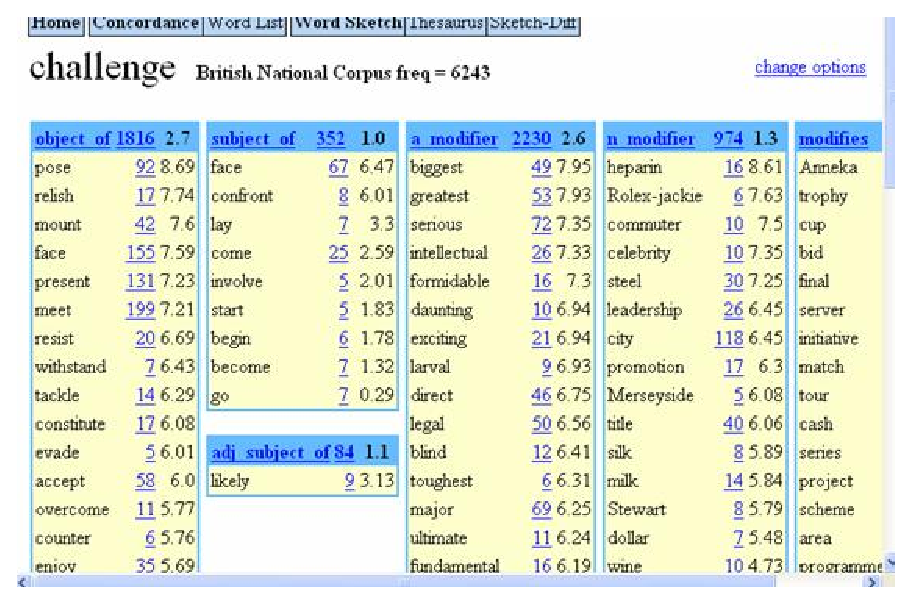
\includegraphics[height=0.98\textheight]{include/ske_wsresults}
% \end{center}


% \myslide{Creating a Word Sketch}

% \begin{itemize}
% \item Each column show the words that typically combine with challenge in a particular grammatical relations (or "gramrels").
%   \begin{itemize}
%   \item object\_of, subject\_ of, modifying, modifies, and/or
%   \item different relations for different parts of speech
%   \end{itemize}
% \item words are listed in  order of statistical significance (logDice)
% \item word sketches can only be made for relatively frequent words
% \end{itemize}

% \myslide{Similarity Score: logDice}
% \lurl{www.fi.muni.cz/usr/sojka/download/raslan2008/13.pdf}
% \begin{itemize}
% \item  Dice coefficient: $D = \frac{2f_{xy}}{f_x+f_y} = \frac{2|x\cap y|}{|x|+|y|}$
% (useful but very low values)
% \item Recalibrate to: \blu{logDice} = $14 + log_2D = 14 + log_2\frac{2f_{xy}}{f_x+f_y}$
%   \begin{itemize}
%   \item Theoretical maximum is 14, in case when all occurrences of X
%     an Y co-occur. Usually the value is less then 10.
% \item Value 0 means there is less than 1 co-occurrence of XY per 16,000 X or
% 16,000 Y. We can say that negative values means there is no statistical
% significance of XY collocation.
% \item Comparing two scores, plus 1 point means twice as often collocation, plus
% 7 points means roughly 100 times frequent collocation.
% \item The score does not depend on the total size of a corpus. The score combines
% relative frequencies of XY in relation to X and Y.
% \end{itemize}
% \end{itemize}


% \myslide{Sketch Differences}
% \lurl{}
% \begin{itemize}
% \item  Sketch Difference is a neat way of comparing two very similar words. It shows:
%   \begin{itemize}
%   \item those patterns and combinations that the two items have in common
%   \item those that mainly appear with on or the other
%   \end{itemize}
% \item Especially useful for showing the differences between similar words
% \end{itemize}

% \myslide{Sketch Difference: \textit{clever/intelligent}}
% \begin{center}
%   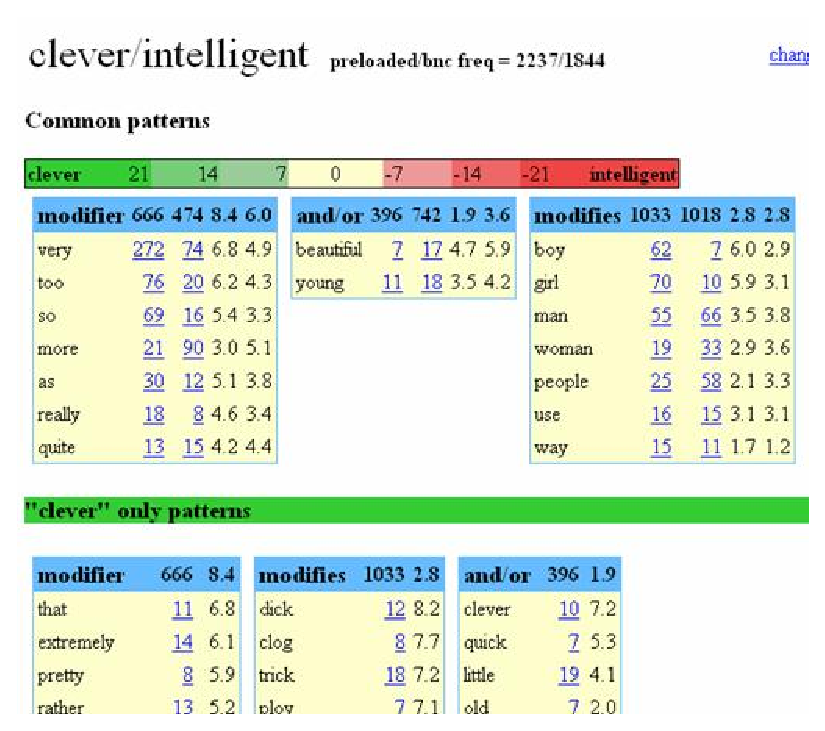
\includegraphics[height=0.98\textheight]{include/ske_sketchdiff}
% \end{center}

\section{DIY Corpora}

\myslide{Why build your own?}

\begin{enumerate}
\item Decide what you want to study
\\ see if you can do it with existing resources
\\ No \frownie
\item Collect data that fits your needs
  \begin{itemize}
  \item Speech (expensive)
  \item Text (easy to get, hard to do legally)
  \end{itemize}
\item Process it
  \begin{itemize}
  \item Clean up
  \item Mark up (what do we know about the data originally)
  \item Annotation (what will we add to it)
  \end{itemize}
\end{enumerate}

\myslide{Collecting Text}

Some ways to collect text:

\begin{itemize}\addtolength{\itemsep}{-1ex}
\item Word-processed texts: save as a text only file
\item Keyboard entry: speech transcription, students' handwritten essays, etc.
\item Scanning: copyright protected novels, latest magazines, etc.
\item CD-ROM: newspaper, encyclopaedia, ICAME, etc.
\item Internet resources: email, chat, public documents, newspapers, magazines etc.
\item  Text archives: copyright free (old) novels, essays, etc.
\item Copying from a large corpus: e.g. using sections of the BNC
\end{itemize}

\myslide{Recent Trends}
\MyLogo{Moving to Open Data}
\begin{itemize}
\item Government Documents (proceedings, publications)
\item Open source documents (manuals, wikipedia)
\item Social Media:  Blogs and twitter
\end{itemize}

\myslide{Web as Corpus}
\myslide{Two Approaches to using the Web as a Corpus}
\begin{itemize}
\item \blu{Direct Query}: Search Engine as Query tool and WWW as corpus?
\\  (Objection: Results are not reliable)
\begin{itemize}
\item Population and exact hit counts are unknown → no statistics
possible.
\item Indexing does not allow to draw conclusions on the data.
\item[\Bad] Google is missing functionalities that linguists /
lexicographers would like to have.
\end{itemize}
\item \blu{Web Sample}: Use search engine to download data from the
net and build a corpus from it.
\begin{itemize}
\item known size and exact hit counts → statistics possible.
\item people can draw conclusions over the included text types.
\item (limited) control over the content.
\item[\Bad] sparser data
\end{itemize}
\end{itemize}

\myslide{Direct Query}
\begin{itemize}
\item Accessible through search engines (Google API, Yahoo API, Scripts)

\item Document counts are shown to correlate directly with ``real''
  frequencies (Keller 2003), so search engines can help - but...
  \begin{itemize}
  \item lots of repetitions of the same text (not representative)
  \item very limited query precision (no upper/lower case, no punctuation...)
  \item only estimated counts, often hard to reproduce exactly
  \item different queries give wildly different numbers
  \end{itemize}
\end{itemize}

\myslide{Web Sample}
\MyLogo{}
\begin{itemize}
\item Extracting and filtering web documents to create linguistically
  annotated corpora (Kilgarriff 2006)
  \begin{itemize}
  \item gather documents for different topics (balance!)
  \item exclude documents which cannot be preprocessed with available
    tools (here taggers and lemmatizers)
  \item exclude documents which seem irrelevant for a corpus (too short or
    too long, word lists,...)
  \item do this for several languages and make the corpora available
  \end{itemize}
\end{itemize}


\myslide{Building Internet Corpora: Outline}
\MyLogo{\url{http://corpus.leeds.ac.uk/internet.html}}

\begin{enumerate}
\item Select Seed Words (500)
\item Combine to form multiple queries (6,000)
\item Query a search engine and retrieve the URLs (50,000)
\item Download the files from the URLS (100,000,000 words)
\item Postprocess the data (encoding; cleanup; tagging and parsing)
\end{enumerate}

Sharoff, S (2006) Creating general-purpose corpora using automated search engine queries. In M. Baroni, S. Bernardini (eds.) WaCky! Working papers on the Web as Corpus, Bologna, 2006.



\myslide{Post-processing}
\begin{itemize}
\item Filter documents by size
  \begin{itemize}
  \item Small documents ($<5KB$) contain very little real text
  \item Large documents ($>200KB$) tend to be indices, catalogues, lists, etc.
  \end{itemize}
\item Remove perfect duplicates
  \begin{itemize}
  \item Actually, removed both the original \& the duplicate:
  \item[\ldots] tend to be warning messages 
  \end{itemize}
\end{itemize}

\myslide{Boilerplate stripping}
\begin{itemize}
\item \blu{Boilerplate}: HTML markup, javascript, other non-linguistic
  material
\item Removing boilerplate information is crucial to obtaining
  linguistic data only
  \begin{itemize}
  \item Content-rich sections of a document will have a low 
    html tag density
  \item Boilerplate sections have a wealth of html
  \item This heuristic is ``relatively independent of language and
    crawling strategy''
  \end{itemize}
\item If a text does not have enough function words, it is likely
non-linguistic material (e.g., a list)
\begin{itemize}
\item Require at least 10 function word types and 30 tokens on a page
\item[\ldots]  which must make up at least 25\% of the total
words
\end{itemize}
\end{itemize}

\myslide{Near-duplicate detection}
\begin{itemize}
\item Take \blu{fingerprints}' of a fixed number of randomly-selected $n$-grams (ignoring function words)
  \begin{itemize}
  \item e.g., extract 25 5-grams from each document
  \end{itemize}
\item Near-duplicates have a high overlap
 \begin{itemize}
 \item e.g., at least 2 5-grams in common
 \end{itemize}
\end{itemize}

%%% FIXME define ngrams

\myslide{Linguistic Post-processing}


\begin{itemize}
\item Prepare the  data  for searching:
  \begin{itemize}
  \item Run a POS tagger over it
  \item Clean the documents further, using POS tags
    \begin{itemize}
    \item Where the POS tag distribution is unusual,
    \item[\ldots] perform another round of anomalous document
finding
\item Look for problematic (erroneous) POS tags and
remove those documents
\item Use cues such as number of unrecognized words,
proporition of words with upper-case initial letters, \ldots
\end{itemize}
\end{itemize}
\item Index the document by word, POS and lemma
\end{itemize}


\myslide{Internet Corpora Summary}
\MyLogo{}
 
\begin{itemize}
\item The web can be used as a corpus
  \begin{itemize}
  \item Direct access
    \begin{itemize}
    \item Fast and convenient
    \item Huge amounts of data
    \item[\Bad] unreliable counts 
    \end{itemize}
  \item Web sample
    \begin{itemize}
    \item Control over the sample
    \item Some setup costs (semi-automated)
    \item[\Bad] Less data 
    \end{itemize}
  \end{itemize}
\item Richer data than a compiled corpus
\item[\Bad] Less balanced, less markup
\end{itemize}



% \myslide{Corpus Tools}

% \begin{itemize}
% \item BNY: 
% \item Sketch Engine \url{https://trac.sketchengine.co.uk/}
% \item Web as Corpus: \url{http://webascorpus.org/searchwc.html}
% \item Internet Corpora: \url{http://corpus.leeds.ac.uk/internet.html}
% \item Google Ngrams: \url{http://ngrams.googlelabs.com/}
% \item Natural Language Tool Kit: \url{http://www.nltk.org/}
% \end{itemize}

\section{Processing Raw Text}

\myslide{Language Identification}

\begin{itemize}

\item Given a document and a list of possible languages, in
  what language was the document written? (e.g.\ English, German, Japanese, Uyghur, ...)
\item Language identification provides us with the means to
  automatically ``discover'' web data to convert into a corpus over
  which to learn linguistic (lexical) properties
\item Main Approaches
\begin{itemize}
\item Linguistically-grounded methods
  \begin{itemize}
  \item Diacritics/Characters
  \item Character $n$-grams
  \item Stop words
  \end{itemize}
\item Statistical Methods
\item Context (under \url{.jp} or \url{.ko}?)
\end{itemize}


\end{itemize}

\myslide{Normalization}

\begin{itemize}
\item Extracting text from various documents
\item Segmenting continuous text
\item Number Normalization:  
  \eng{\$700K}, \eng{\$700,000}, \eng{0.7 million dollars},  \ldots
\item Date Normalization:   \eng{2000AD, 1421AH,  Heisei 12, \ldots} 
\item Stripping stop words
\item Lemmatization:  \textit{produces}   \infers \textit{produce}
\item Stemming:  \textit{producer}   \infers \textit{produc}; \textit{produces}   \infers \textit{produc}
\item Decompounding: \textit{zonnecel}  \infers \textit{zon cel}
\end{itemize}


\section{Relational Databases \\ and SQL}

\myslide{Many corpora are stored as Relational Data-Bases}

\begin{itemize}
\item Data is stored in \txx{Table}s (or relations)
  \begin{itemize}
  \item \txx{attribute}s are  \txx{column}s
  \item \txx{record}s are \txx{row}s
  \end{itemize}
    \item Tables can be joined together
  \begin{itemize}
  \item If they share a common column
  \end{itemize}
\item Data can be retrieved with \txx{Queries}
  \begin{itemize}
  \item Properly written these can be very fast
  \end{itemize}
\end{itemize}
\txx{Structured Query Language} (SQL) is a special-purpose
programming language designed for managing data held in a relational
database management system (RDBMS)


\myslide{Example tables}

\begin{tabular}{lllll}
  \multicolumn{2}{c}{TABLE: sent} \\
  sid & sent \\ \hline
  INTEGER & STRING \\ \hline
  1   & Does this work? \\
  2   & I hope so. \\
\end{tabular}


\begin{tabular}{lllll}
  \multicolumn{5}{c}{TABLE: word} \\
  sid & wid & word & pos& lemma \\ \hline
  INTEGER &INTEGER & STRING& STRING & STRING \\ \hline
  1   &  1 & Does & VBZ & do \\
  1   &  2 & this & DT & this \\
  1   &  3 & work & NN & work \\
  1   &  4 & ?    & . & ? \\
  2   &  1 & I & PRN & i \\
  \ldots
\end{tabular}


\myslide{Select-From-Where}

\begin{itemize} \addtolength{\itemsep}{-1ex}
\item The simplest query
  \begin{itemize}
  \item SELECT desired attributes (columns)
  \item FROM one or more tables
  \item WHERE condition applies about the records  in the tables
  \end{itemize}
\item What lemmas are there associated with the word \eng{does}?
\begin{verbatim}
SELECT word, lemma
FROM word
WHERE word = 'does'
\end{verbatim}

  \begin{tabular}{ll}
    \textbf{word} & \textbf{lemma} \\ \hline
    does & do \\
    does & do \\
    does & doe \\
    \ldots
  \end{tabular}
\end{itemize}

\myslide{How does it work?}

\begin{itemize}
\item Begin with the table in the FROM clause.
\item Apply the selection indicated by the WHERE clause.
\item Select only those parts indicated by the SELECT clause.
\end{itemize}


Note: each query ends with a semicolon ``;'', not shown in the example

\myslide{* in SELECT}

\begin{itemize}
\item When there is one relation in the FROM clause, * in the SELECT clause stands for “all attributes of this relation.”
\item What information is there associated with the word \eng{does}?
\begin{verbatim}
SELECT *
FROM word
WHERE word = 'does'
\end{verbatim}
  \begin{tabular}{lllll}
   \textbf{sid} & \textbf{wid} &  \textbf{word} & \textbf{pos} & \textbf{lemma} \ldots \\ \hline
    10 & 1 & does & VBZ & do \\
    11 & 7 & does & VBZ & do \\
    14 & 4 & does & NNS & doe \\
    \ldots
  \end{tabular}
\end{itemize}

\myslide{You can rename things}

\begin{itemize}
\item What information is there associated with the word \eng{does}?
\begin{verbatim}
SELECT word AS surface, lemma AS indexform, pos
FROM word
WHERE word = 'does'
\end{verbatim}
  \begin{tabular}{lllll}
    \textbf{surface}  & \textbf{indexform}  &  \textbf{pos} \\ \hline
    does & do  & VBZ \\
    does & do  & VBZ \\
    does & doe & NNS \\
    \ldots
  \end{tabular}
\end{itemize}

\myslide{You can sort things}

\begin{itemize}\addtolength{\itemsep}{-1ex}
\item What information is there associated with the word \eng{does}, sorted by POS?
\begin{verbatim}
SELECT word AS surface, lemma AS indexform, pos
FROM word
WHERE word = 'does'
ORDER BY pos DESC
\end{verbatim}
  \begin{tabular}{lllll}
    \textbf{surface}  & \textbf{indexform}  &  \textbf{pos} \\ \hline
    does & do  & VBZ \\
    does & do  & VBZ \\
    does & doe & NNS \\
    \ldots
  \end{tabular}
\item You can specify the order with \texttt{DESC} or \texttt{ASC} (default)
\item You can order by multiple things: \texttt{ORDER BY pos, LENGTH(word)}
\end{itemize}

\myslide{And add new things}

\begin{itemize}\addtolength{\itemsep}{-1ex}
\item What is the lemma, its length and pos associated with the word \eng{does}?
\begin{verbatim}
SELECT  lemma, LENGTH(lemma) AS length, pos
FROM word
WHERE word = 'does'
\end{verbatim}
  \begin{tabular}{lllll}
    \textbf{lemma}  & \textbf{length}  &  \textbf{pos} \\ \hline
    do  & 2 &  VBZ \\
    do  & 2 &  VBZ \\
    doe & 3 &  NNS \\
    \ldots
  \end{tabular}
\item strings:  \texttt{LENGTH(), LOWER(), UPPER(), TRIM(), LTRIM(),
    RTRIM()}
  \\ \texttt{SUBSTR(str,from, len), REPLACE(str, from, into)}
\item numbers:  \texttt{ROUND(num,digits=0), ABS(num)}
\end{itemize}

\myslide{Task}

\begin{itemize}
\item Download \texttt{eng.db} and \texttt{cmn.db}
\item Start the sqlitebrowser
\item Open \eng{eng.db}
  \begin{itemize}
  \item Find all surface forms of \lex{leave}
  \item Find all surface forms of \lex{leave}, and show their length
  \item Find all surface forms of \lex{leave}, ordered from longest to shortest
  \end{itemize}
\end{itemize}

\begin{enumerate}
\item Open the database
\item Look at the database structure
\item Execute SQL
\end{enumerate}

\myslide{You can have complex conditions and limits}

\begin{itemize}
\item Show 5 words that are not the same as their lemmas:
\begin{verbatim}
SELECT  word, lemma, pos
FROM word
WHERE word != lemma
LIMIT 5
\end{verbatim}
  \begin{tabular}{lllll}
    \textbf{word}  & \textbf{lemma}  &  \textbf{pos} \\ \hline
    does  & do &  VBZ \\
    held  & hold &  VBN \\
    does & does &  NNS \\
    Holmes & holmes & NNP \\
    Holmes & holmes & NNP \\
    \ldots
  \end{tabular}
\end{itemize}

\myslide{You can even have simple regular expressions}

\begin{itemize}
\item Show 5 words that include the string \texttt{dog}:
\begin{verbatim}
SELECT  word, lemma, pos
FROM word
WHERE word GLOB '*dog*'
LIMIT 5
\end{verbatim}
  \begin{tabular}{lllll}
    \textbf{word}  & \textbf{lemma}  &  \textbf{pos} \\ \hline
dog-cart   & dog-cart   &  NN      \\  
dog        & dog        &  NN    \\    
dog-       & dog        &  NN   \\     
dog-cart   & dog-cart   &  NN   \\     
dogged     & dog        &  VBD   \\
    \ldots
  \end{tabular}
\end{itemize}

\myslide{Or slightly complicated ones}

\begin{itemize}
\item Show 5 words starting with dog or Dog whose part of speech is not a noun
\begin{verbatim}
SELECT  word, lemma, pos
FROM word
WHERE word GLOB '[dD]og*' AND pos NOT GLOB 'N*'
LIMIT 5
\end{verbatim}
  \begin{tabular}{lllll}
    \textbf{word}  & \textbf{lemma}  &  \textbf{pos} \\ \hline
    dogged  & dog &  VBN \\
  \end{tabular}
\begin{itemize}
\item[*] matches anything
\item[?] matches one or one of anything
\item[{[\ ]}] matches all characters listed (and allows
  \textasciicircum\ for negation and - for ranges)
  \\ e.g., [a-z], [\textasciicircum{}H], 
\end{itemize}
\end{itemize}

\myslide{You can aggregate results}

\begin{itemize}
\item Tell me more about the words
\begin{verbatim}
SELECT COUNT(word), COUNT(DISTINCT word),
       MIN(LENGTH(word)), 
       MAX(LENGTH(word)), AVG(LENGTH(word))
FROM word
\end{verbatim}
  \begin{tabular}{lllll}
    \textbf{count}  & \textbf{distinct} &\textbf{min}  &  \textbf{max} & \textbf{avg} \\ \hline
    77820 & 9485 & 1 & 86 & 4.437
  \end{tabular}
\item  \texttt{MIN(num), AVG(num), MAX(num)} are calculated over the whole set
\item \texttt{DISTINCT} eliminates duplicate records thus fetches only unique records
\end{itemize}

\myslide{You can group things}
\MyLogo{A random word (the first it finds) will be inserted}
\begin{itemize}
\item Tell me more about the words grouped into parts-of-speech
\begin{verbatim}
SELECT pos, word,
       count(word), count(DISTINCT word),
       MIN(LENGTH(word)), 
       MAX(LENGTH(word)), AVG(LENGTH(word))
FROM word
GROUP BY pos
\end{verbatim}
  \begin{tabular}{llrrrrr}
    \textbf{pos} & \textbf{word} & \textbf{count} & \textbf{distinct}  
  & \textbf{min}  &  \textbf{max} & \textbf{avg} \\ \hline
  CC & and  & 2264 & 13 & 2 & 7 & 2.98 \\
  DT & the  & 8256 & 38 & 1 & 7 & 2.74 \\
  EX & There&  243 &  2 & 5 & 5 & 5.00  \\
\ldots
  \end{tabular}
\end{itemize}


\myslide{Task}

\begin{itemize}
\item Which POS has the greatest difference between lemma and word length?
\item Which preposition has a lemma not equal to its surface form?
\item Find the number of words in each POS and sort from most to least
  frequent (for both English and Chinese)
\end{itemize}

\myslide{You can have a list in your condition}

\begin{itemize}
\item Tell me more about common nouns
\begin{verbatim}
SELECT count(word), count(DISTINCT word),
       MIN(LENGTH(word)), 
       MAX(LENGTH(word)), AVG(LENGTH(word))
FROM word
WHERE pos IN ('NN', 'NNS')
\end{verbatim}
  \begin{tabular}{lllll}
    \textbf{count}  & \textbf{distinct} &\textbf{min}  &  \textbf{max} & \textbf{avg} \\ \hline
    14457 & 3593 & 1 & 21 & 6.74
  \end{tabular}
\item  \texttt{MIN(num), AVG(num), MAX(num)} are calculated over the whole set
\item \texttt{DISTINCT} eliminates duplicate records thus fetches only unique records
\end{itemize}

\myslide{This list can be the result of a select!}

\begin{itemize}
\item Tell me more about frequent common nouns
\begin{verbatim}
SELECT count(word), count(DISTINCT word),
       MIN(LENGTH(word)), 
       MAX(LENGTH(word)), AVG(LENGTH(word))
FROM word
WHERE word 
IN (SELECT word
    FROM word
    WHERE POS in ('NN', 'NNS') 
    GROUP BY word
    ORDER BY COUNT(word) DESC
    LIMIT 10)

\end{verbatim}
  \begin{tabular}{lllll}
    \textbf{count}  & \textbf{distinct} &\textbf{min}  &  \textbf{max} & \textbf{avg} \\ \hline
    1096 & 10 & 3 & 10 & 5.13
  \end{tabular}
\item First find the ten most common words, then do things to them
  \begin{itemize}
  \item the trick is to write simple queries first, and then combine them
  \end{itemize}
\item Note that more common words are shorter (as we would expect)
\end{itemize}
\begin{center}
  Now try to do some corpus queries yourself!
\end{center}


\myslide{You can Create Tables}

You tell the database what the data will look like:
\begin{verbatim}
CREATE TABLE word (
    sid INTEGER,
    wid INTEGER,
    word TEXT,
    pos TEXT,
    lemma TEXT,
    cfrom INTEGER,
    cto INTEGER,
    comment TEXT,
    usrname TEXT,			
    PRIMARY KEY (sid, wid),
    FOREIGN KEY(sid) REFERENCES sent(sid)
    );
\end{verbatim}

\myslide{You can Drop Tables}
You tell the database what the data will look like:
\begin{verbatim}
DROP TABLE word;
\end{verbatim}

But be careful, you can't get it back.

\myslide{You can Insert Data}

\begin{verbatim}
INSERT INTO word (sid, wid, word, lemma, pos)  
VALUES (1, 1, 'The', 'the', 'DT');
\end{verbatim}

Normally you would add data using a program, or read it in from some
other file, \ldots

\myslide{You can Update Data}

\begin{verbatim}
UPDATE word SET lemma='a', word='A'
WHERE sid=1,wid=1;
\end{verbatim}

This changes the value permanently for all rows that match the
condition.

\begin{verbatim}
UPDATE word SET pos='ART'
WHERE pos = 'DT';
\end{verbatim}

You can change a lot at a time.

\myslide{You can Delete Data}

\begin{verbatim}
DELETE FROM word WHERE word='gannet';
\end{verbatim}

But be careful, you can't get it back.

\myslide{You can Index Data}

Indexes are special tables that the database can use to speed up data
retrieval.  An index is a pointer to data in a table, think of it as
index in the back of a book.  An index helps to speed up SELECT
queries and WHERE clauses, but it slows down data input, with the
UPDATE and the INSERT statements. Indexes can be created or dropped
with no effect on the data.

\begin{verbatim}
CREATE INDEX word_word_idx ON word (word);
CREATE INDEX word_lemma_idx ON word (lemma);
\end{verbatim}

This makes it possible to look up words and lemmas very fast, but makes the
database bigger.  You normally add them after you have added the
data.  Whether they speed things up or not is an empirical question,
and should be tested.

\myslide{SQL and NLP}


\begin{itemize}
\item RDMS and SQL are the backbone of most data storage
\item There are many implementations:
  \begin{itemize}
  \item SQLite, PostgreSQL, ORACLE, MySQL, MS SQL Server, \ldots
  \item typically share the same core
  \item may have different extensions
  \end{itemize}
\item Text to SQL query is a popular task
  \begin{itemize}
  \item \eng{Which is the longest verb?}
  \item[\ensuremath{\rightarrow}]
\begin{verbatim}
    SELECT word, pos FROM word
    WHERE POS GLOB 'V*' AND
    LENGTH(word) =
    (SELECT MAX(LENGTH(word)) FROM word
    WHERE POS GLOB 'V*');
\end{verbatim}
    
    
  \end{itemize}

\end{itemize}

% \myslide{Acknowledgments}


% \begin{itemize}
%   \item Thanks to Stefan Th. Gries (University of California, Santa
% \end{itemize}



\end{document}


%%% Local Variables: 
%%% coding: utf-8
%%% mode: latex
%%% TeX-PDF-mode: t
%%% TeX-engine: xetex
%%% LaTeX-section-list:  (("myslide" 1))
%%% End: 